\documentclass[a4paper,11pt, oneside]{article}  % document class
\usepackage{geometry}
\geometry{
  inner=20mm,
  outer=20mm,
  top=30mm,
  bottom=25mm %
%  heightrounded,
%  marginparwidth=50pt,
%  marginparsep=17pt,
%  headsep=20pt
}
\usepackage[english]{babel}
\usepackage{hyperref}
%pacchetto
\usepackage{import, multicol,lipsum}  % package
\setlength{\columnsep}{1cm}

\usepackage[utf8]{inputenc} % accenti facili
\usepackage[T1]{fontenc}
\usepackage{subcaption}
\usepackage{pifont}
\usepackage{url}
\hypersetup{
	colorlinks=true,
	linkcolor=blue,
	filecolor=magenta,      
	urlcolor=blue
}
\usepackage{graphicx, color, blindtext}
\usepackage{textcomp, makeidx, times}
\usepackage{amsthm, amsmath, amssymb, amsfonts, mathtools} % math
\usepackage[mathscr]{eucal}		
\usepackage[nottoc]{tocbibind} 
\usepackage{pgfplots, parskip}
\usepackage{afterpage, ifthen}
\usepackage{enumitem}
\pgfplotsset{compat=newest}
\usepackage{graphicx} % immagini
\usepackage{wrapfig}
%\graphicspath{ {image/} } % path cartella delle immagini
\usepackage{tikz} %graph
\usetikzlibrary{arrows,automata}
\usetikzlibrary{automata,arrows,positioning,calc,matrix}
\usepackage[linesnumbered,ruled,vlined]{algorithm2e}
\usepackage{booktabs}
\usepackage{colortbl}
\usepackage{siunitx}
\usepackage{tabularx, tabu}
\usepackage{relsize}
\usepackage{makecell, caption, chngcntr}
\usepackage{bbm}
\usepackage{diffcoeff}
\RequirePackage{fix-cm}


%
%____________________________________________________________________________________________________________________________
%____________________________________________________________________________________________________________________________
%____________________________________________________________________________________________________________________________
%____________________________________________________________________________________________________________________________
% INIZIO
\begin{document}

\setcounter{secnumdepth}{2}
\pagestyle{plain} % stile pagina (header, numerazioni)

\centerline {
\includegraphics[width=2cm]{logo.jpg}}
\begin{center}
Università degli Studi di Torino - M.Sc.  in Stochastic and Data Science - A.Y.  2021/2022 \\
\Large { Final project of Statistical Machine Learning (MAT0043)}
\line(1,0){450}\\ 
\vspace{0.4cm} 
{ \huge \textbf{Gene selection for cancer type classification} }
\vspace{0.1cm}
\line(1,0){450} \\
\end{center}

%____________________________________________________________________________________________________________________________
% ABSTRACT

From the DepMap Portal website\footnote{DepMap Portal: \url{https://depmap.org/portal/} } we downloaded a dataset containing 1032 cancerous cells whose $\sim 17000$ columns represent the probability that the inhibition of that given gene stops the growth of the cancer.  The label of each cell line refers to the cancer type and is a categorical factor which can assume 10 values: Eye, Gastrointestinal,  Gynecologic,  Musculoskeletal,  Neurological,  Breast,  Head-Neck,  Hematologic,  Genitourinary,  Lung.  The project then focuses on the problem of Genes Selection for Cancer Classification,  i.e.  finding a relatively small number of genes to predict the type of cancer of a given tumorous cell.  To this aim we explored in detail three Features Selection algorithms: Random Forests combined with Feature Importance,  Lasso-SVM and Neural Networks (NN) combined with Permutation Importance.  We repeated these procedures on three distinct classification tasks: blood cancer vs rest,  lung cancer vs rest and multiclass.  Apart from the cases involving lung data,  we achieved satisfying classification accuracies on the whole dataset and we were able to select about 100-200 genes from the starting ~17000 ones.  We then used these features to fit reduced versions of the previous classifiers and obtained classification accuracies which range from $67\%$ to $98\%$.  We then concluded that the possibility of classifying the type of cancer from an extremely reduced numbers of genes depends on the cancer type itself.  In particular,  these methodologies worked incredibly well on blood cancer for which we achieved almost $100\%$ accuracy with the reduced classifier while failed miserably on lung cancer.  


%The purpose of our project is to work on a high-dimensional genomics data and find a relatively small number of genes to predict the cancer type of a given tumorous cells. This is known as Genes Selection for Cancer Classification and it is in line with many up-to-date problems of applied medicine.  Our dataset contains $1.032$ cells and their knock-out probabilities, i.e. the probabilities of stopping the growth of cancer by inhibiting one of the $\sim 17.000$ genes. Each cell line is characterised by one of 10 possible cancer labels: Eye, Gastrointestinal, Gynecologic,  Musculoskeletal, Neurological, Breast, Head-Neck, Hematologic, Genitourinary and, finally, Lung. We explore in details three Features Selection algorithms: Random Forests (RF) combined with Feature Importance, Lasso-SVM and Neural Networks (NN) combined with Permutation Importance. We have studied two binary classifications (Blood-cancer vs. All, Lung-cancer vs. All) and multiclassification. Besides lung models, we achieves satisfying classification accuracies and we are able to select about $100$-$200$ genes from the initial $\sim 17.000$ ones. Models fitted on such genes obtain classification accuracies ranging from $67\%$ to $98\%$. Therefore, it seems that classifying cancer type from an extremely small set of genes depends on the cancer type itself. 


\section{Introduction}
Cancer is a complex disease characterized by the uncontrolled growth of abnormal cells anywhere in the body. These abnormal cells are extremely invasive and we usually identify them with the name of their original tissue (for instance, breast cancer,  lung cancer,  brain cancer, etc.).  In recent years,  medicine has made a great step forward in finding new and efficient therapies for different diseases and cancer is one of them.  In particular,  thanks to numerous advances in technology,  collecting huge amount of data is no longer an issue,  so that one can exploit such information to define personalized treatments for patients.  In this regards,  the DepMap project and,  in particular,  the Achilles project aim to use genome-wide screens to collect data regarding mutations of cancerous cells,  identify essential genes and report vulnerabilities across hundreds of human cancers.  \\
 
Many researches are currently using DepMap datasets to identify relatively small sets of genes which are responsible of cancers growth. This procedure is often driven by medical knowledge,  which we do not possess,  together with some rough measures of importance.  Being Maths student,  we instead base our research on statistical models only  and on the hypothesis that if a given classifier is able to distinguish different types of cancer then the most relevant genes are the most important features for that given classifier (the meaning of "important features" will be clarified later).  This finding would have outstanding implications in the medical field such building faster diagnosis tools and synthesizing less toxic drugs that target only these specific genes. 


\section{Dataset}
We used two public datasets from the DepMap Portal website\footnote{Download dataset from DepMap:  \url{https://depmap.org/portal/download/}:}
\begin{itemize}
	\item[D1] \textit{CRISPR\_gene\_dependency.csv},  which contains $1.032$ cancer cell lines characterised by $17.393$ gene scoring results
	\item[D2] \textit{sample\_info.csv}, which contains cell lines information,  such as primary disease and sample collection site
\end{itemize}
Data were collected from real patients and successively processed,  so that element $(i, j)$ of this $(1.032 \times 17.393)$-data frame is the probability that knocking out gene $j$ has a real depletion effect on the $i$-th cell.  In order to work on a labeled datates and perform classification we associated the primary disease (i.e.  the name of the cancer type) to each cell line performing an inner join of D1 and D2 on the DepMap ID.  Then,  we dedicated ourselves in data cleaning: we removed missing values,  which affected only 10 rows,  and all instances labeled as "Non Cancerous" and "Engineered".  


\begin{wrapfigure}{r}{0.65\textwidth}
	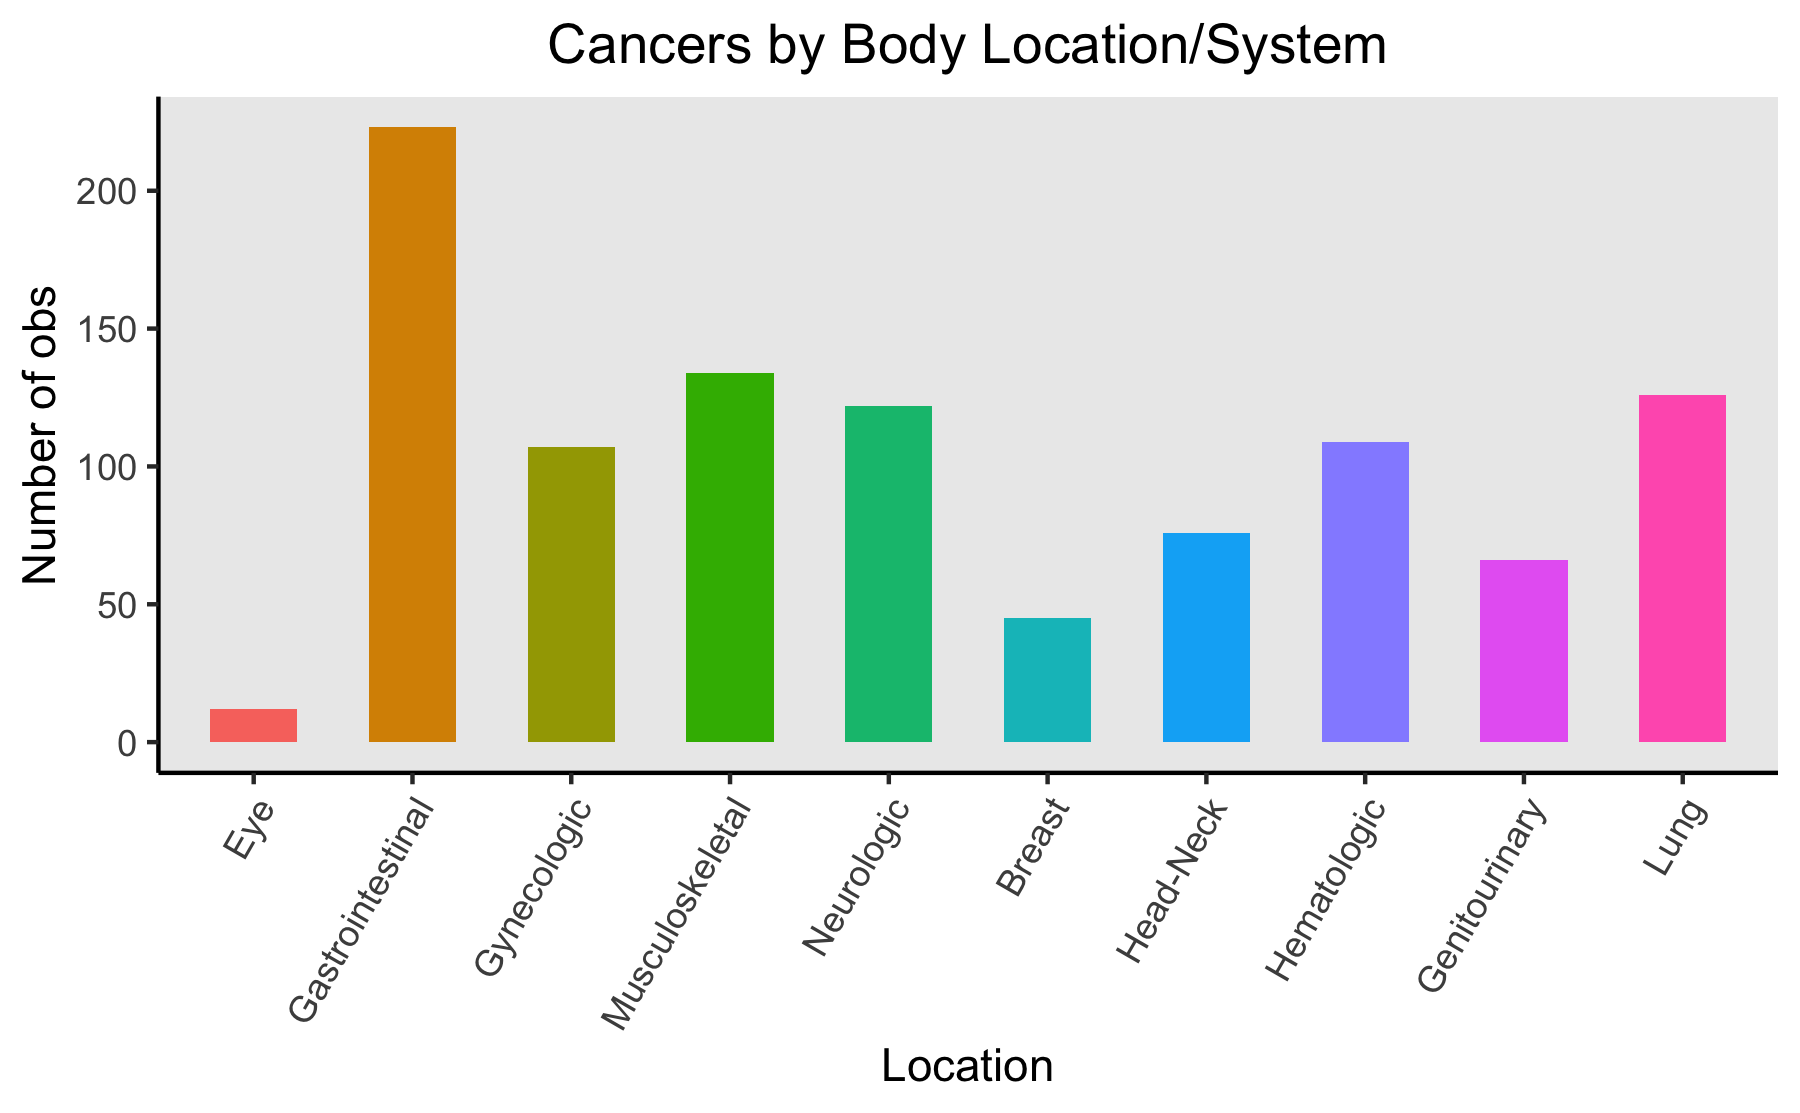
\includegraphics[width=0.65\textwidth]{plot1.png}
	\captionof{figure}{Cancer classes}\label{fig1}
\end{wrapfigure}

We then group the various cancer types in 10 classes according to common medical knowledge\footnote{Cancer types grouped by body location: \url{https://www.cancer.gov/types/by-body-location}} and we obtain the groupings as reported in Figure \ref{fig1}.  "Eye" is the smallest one as there are only $16$ observations and $5$ of them are labeled while "Gastrointestinal" is the largest class as it comprehends $7$ types of cancer,  making this group quite heterogeneous.  The project was then developed by investigating two binary classification problems,  Blood vs Rest and Lung vs Rest,  and the multiclass problem.  The choice of Lung was dictated by the fact that it is the most numerous class while the choice of Blood was driven by some underlying biological knowledge. In fact,  Blood cancer is quite different from other tumors because
\begin{itemize}
	\item blood is in the whole body
	\item Leukemia, Lymphom and Myeloma are the main kinds of cancer but they all affect white blood cells
	\item not all blood cancers require a treatment, just periodical monitoring
\end{itemize} 


\section{Methods}
\subsection{Random Forests}

\subsection{SVM-Lasso}

\subsection{Neural Networks}


\section{Results}


\section{Conclusion and future works}


%\end{multicols}
\end{document}